\documentclass[10pt, export, handout]{beamer}

\usepackage[utf8]{inputenc}
\usepackage[T1]{fontenc}

\usepackage{standalone}
    
\usepackage[acronym]{glossaries}
    
\usepackage{enumitem}
    
\usepackage{multirow}
\usepackage{multicol}
    
\usepackage{array}
\newcolumntype{x}[1]{>{\centering\let\newline\\\arraybackslash\hspace{0pt}}p{#1}}
\usepackage{booktabs, colortbl}
    
\usepackage{siunitx}
\usepackage{mathrsfs, amsmath}

\usepackage{graphicx}
\usepackage{subcaption}
\usepackage[font={small, color=IGNDarkGrey}, labelformat=empty]{caption}
\DeclareCaptionFont{footnotesize}{\footnotesize}
\usepackage[font={footnotesize, color=IGNDarkGrey}, labelformat=empty]{subcaption}
\usepackage{adjustbox}

\usepackage{tikz}
\usetikzlibrary{calc, 3d, shapes, arrows, shadows, decorations}

\usepackage{pgfplots, pgfplotstable}


\usepackage{pifont, textcomp}
\newcommand{\cmark}{{\color{green} \ding{51}}}%
\newcommand{\xmark}{{\color{red} \ding{55}}}%

\definecolor{Moins4}{RGB}{183,10,10}
\definecolor{Moins3}{RGB}{255,0,0}
\definecolor{Moins2}{RGB}{255,122,12}
\definecolor{Moins1}{RGB}{255,181,12}
\definecolor{Zero}{RGB}{255,255,255}
\definecolor{Plus1}{RGB}{58,255,12}
\definecolor{Plus2}{RGB}{58,155,12}


\usepackage{hyperref}

\usepackage[useregional]{datetime2}
    
\usepackage[
        backend=biber,
        style=alphabetic,
        backref=true,
        sorting=none,
        autocite=footnote,
        maxnames=2,
        hyperref=true,
        natbib=false,
        abbreviate=true,
        doi=false,
        isbn=false,
        url=false
    ]{biblatex}
\addbibresource{references.bib}
\setbeamerfont{footnote}{size=\tiny}


\usetheme{ign}


\newacronym{acr::lod}{LoD}{Level of Detail}
\newacronym{acr::elod}{eLoD}{evaluation Level of Detail}
\newacronym{acr::lidar}{LiDAR}{Light Detection and Ranging}
\newacronym{acr::dsm}{DSM}{Digital Surface Model}
\newacronym{acr::gui}{GUI}{Graphical User Interface}

\title{Reconstructed 3D building model evaluation}
\subtitle{the forgotten step}
\date{\tiny\DTMdisplaydate{2019}{4}{19}{5}}
\author{\scriptsize \underline{\textbf{Oussama Ennafii}} \inst{1, 2}, Arnaud Le Bris \inst{1}, Cl\'ement Mallet \inst{1}, Florent Lafarge \inst{2}}
\institute{\scriptsize \inst{1} Univ. Paris Est, LaSTIG STRUDEL, IGN, ENSG\\ \scriptsize \inst{2} Inria, TITANE}

\begin{document}
    \begin{frame}[plain]
        \titlepage{}
    \end{frame}

    \section{Introduction}
        \begin{frame}{Context: 3D model vs. 3D mesh}
            \begin{figure}
                \begin{center}
                    \begin{subfigure}{\textwidth}
                        \begin{center}
                            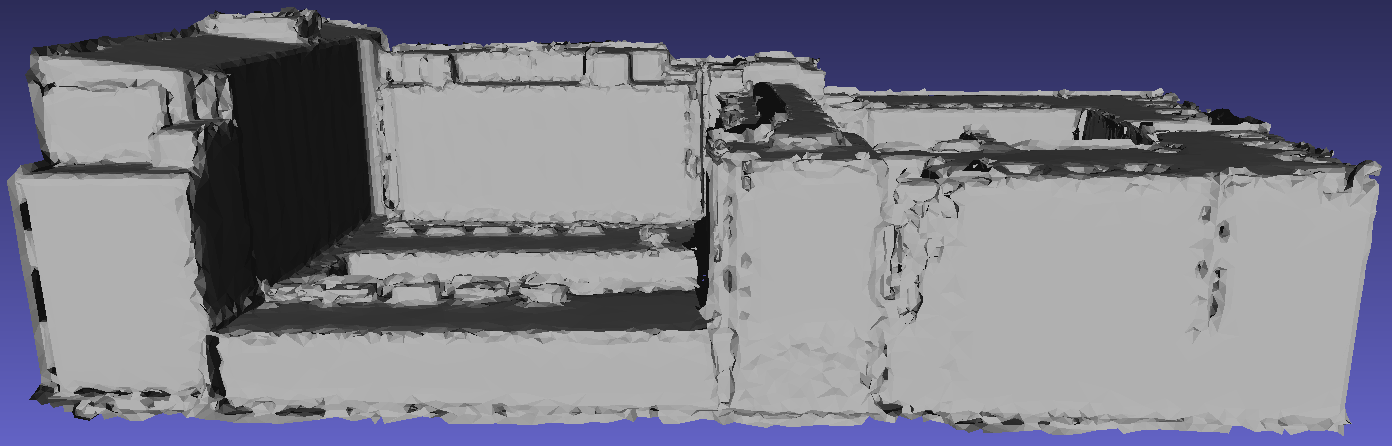
\includegraphics[height=.28\textheight]{images/difference_mesh_model/bercy_building_mesh_1_e5}
                            \caption{\underline{3D mesh} of a building surface ($\approx$ \num[output-exponent-marker = \text{e}]{1e5} triangles).}
                        \end{center}
                    \end{subfigure}
                    \\
                    \begin{subfigure}{\textwidth}
                        \begin{center}
                            \includestandalone[mode=buildnew, height=.28\textheight]{ground_truth_model}
                            \caption{Building \underline{3D polyhedral model} ($\approx$ 800 facets).}
                        \end{center}
                    \end{subfigure}
                    \caption{Different model schemes of a building ($\approx$ \SI{139 x 71 x 23}{\metre}).}
                \end{center}
            \end{figure}
        \end{frame}
        \begin{frame}{Motivation}
            \only<1-4|handout:1>{
                \begin{itemize}[label=$\blacktriangleright$, font=\color{IGNGreen}, itemsep=2em]
                    \item<1-> Automatic urban modeling: an \underline{active} research area \footfullcite{Musialski2012};
                    \item<2-> Results \textcolor{IGNGreen}{seamless} but \textcolor{IGNRed}{lack generality} and \textcolor{IGNRed}{often erroneous} \footfullcite{rottensteiner2014results};
                    \begin{itemize}[label=$\longrightarrow$]
                        \item<3-> labourious manual corrections: $\approx$ \SI{2}{\hour\per\km\squared} per expert.
                    \end{itemize}
                    \item<4-> Urban 3D model semantic diagnostic \textcolor{IGNRed}{not well studied} \footfullcite{boudet2006supervised}\footfullcite{Michelin2013};
                \end{itemize}
            }
            \only<5-|handout:2>{
                \begin{block}{\textcolor{purple}{\textbf{Goal}}}
                    \underline{Detect} and \underline{describe} semantic errors that affect building 3D models.
                \end{block}
                ~\\
                \begin{itemize}[label=$\blacktriangleright$, font=\color{IGNGreen}, itemsep=2em]
                    \item<6-> Semantic errors \textbf{independent} from \underline{reconstruction methods} and \underline{urban scenes}.
                    \item<7-> \underline{Transferability}, and \underline{scalability}, of the evaluation method.
                \end{itemize}
            }
        \end{frame}
        \begin{frame}{Potential use}
            \begin{minipage}[0.2\textheight]{\textwidth}
                \begin{columns}[T]
                    \begin{column}{0.48\textwidth}
                        \begin{itemize}[label=$\blacktriangleright$, font=\color{IGNGreen}, itemsep=2em]
                            \item<1-> Change detection;
                            \item<2-> Urban models correction;
                            \item<3-> Urban reconstruction method evaluation;
                            \item<4-> Crowd reconstruction quality assessment.
                        \end{itemize}
                    \end{column}
                    \begin{column}{0.48\textwidth}
                        \only<1|handout:0>{
                            \begin{figure}
                                \begin{center}
                                    \begin{subfigure}{.8\textwidth}
                                        \begin{flushright}
                                            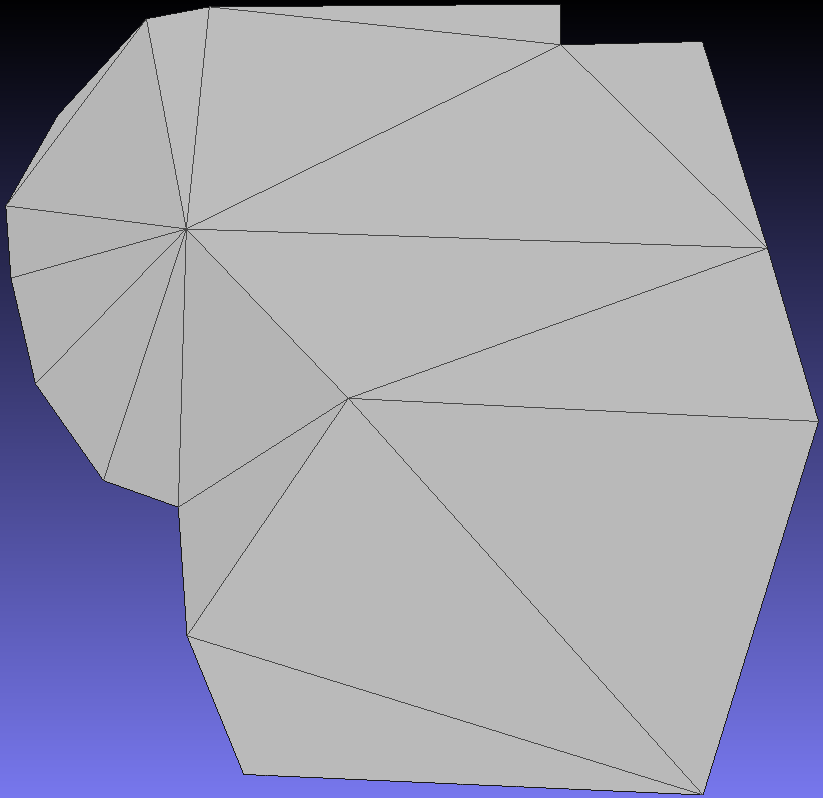
\includegraphics[width=.55\textwidth]{images/use/top_building_change_before}
                                        \end{flushright}
                                    \end{subfigure}
                                    \begin{subfigure}{.8\textwidth}
                                        \begin{flushright}
                                            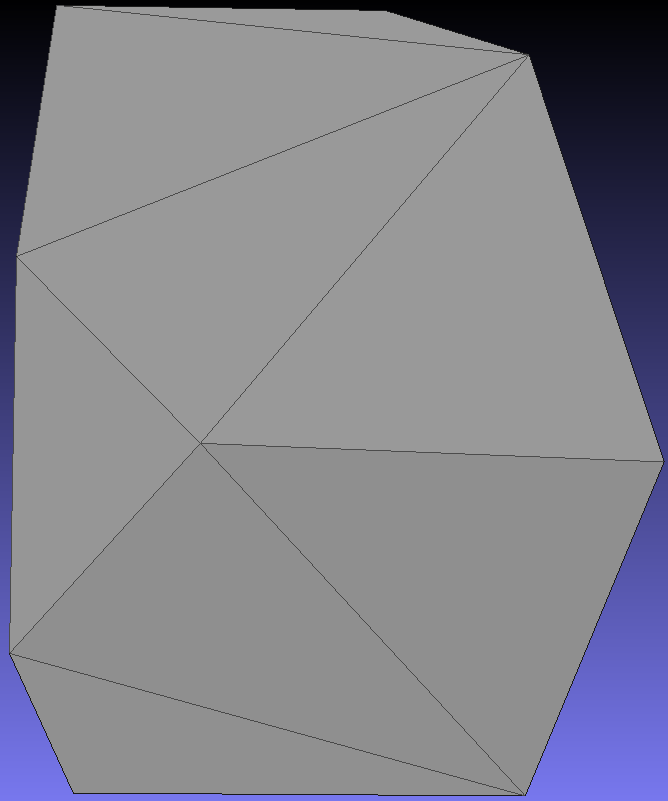
\includegraphics[width=.4447\textwidth]{images/use/top_building_change_after}                                            
                                        \end{flushright}
                                    \end{subfigure}
                                \end{center}
                            \end{figure}
                        }
                        \only<2|handout:0>{
                            \begin{figure}
                                \begin{center}
                                    \begin{subfigure}{.8\textwidth}
                                        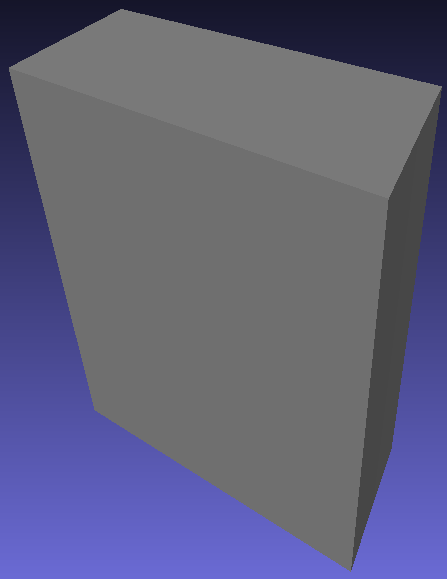
\includegraphics[width=\textwidth]{images/use/incorrect_model}
                                    \end{subfigure}
                                    \begin{subfigure}{.8\textwidth}
                                        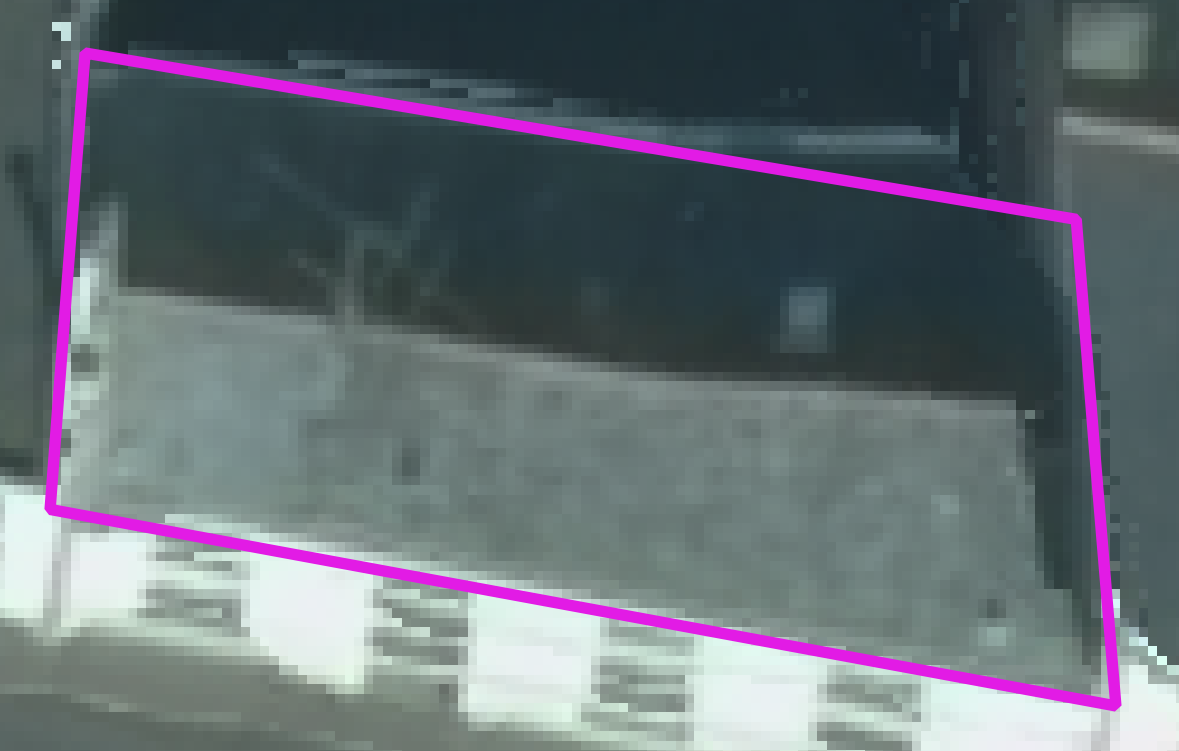
\includegraphics[width=\textwidth]{images/use/incorrect_proj}
                                    \end{subfigure}
                                \end{center}
                            \end{figure}
                        }
                        \only<3|handout:0>{
                            \begin{figure}
                                \begin{center}
                                    \begin{subfigure}{.8\textwidth}
                                        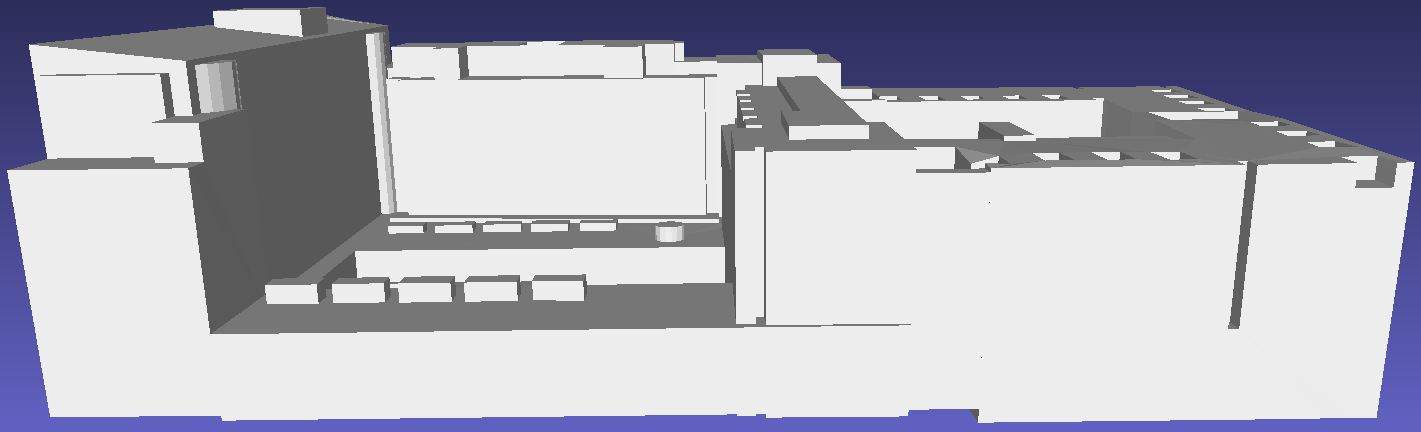
\includegraphics[width=\textwidth]{images/difference_mesh_model/ground_truth}
                                    \end{subfigure}
                                    \begin{subfigure}{.8\textwidth}
                                        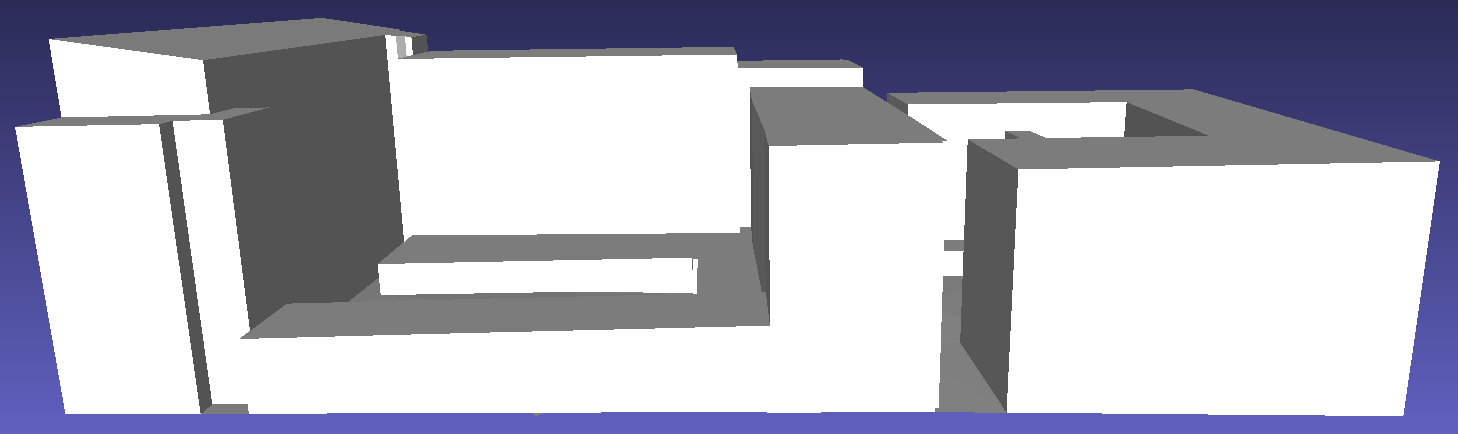
\includegraphics[width=\textwidth]{images/use/bati3d_bercy}
                                    \end{subfigure}
                                \end{center}
                            \end{figure}
                        }
                        \only<4|handout:0>{
                            \begin{figure}
                                \begin{center}
                                    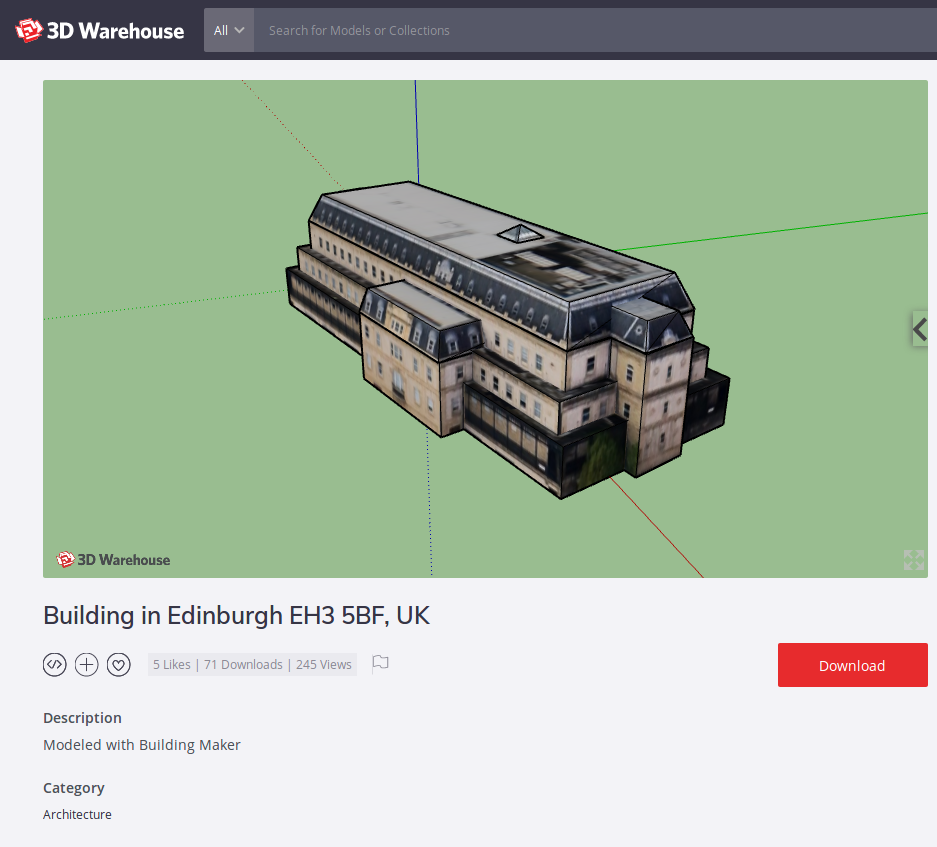
\includegraphics[width=\textwidth]{images/use/crowdsourcing}
                                \end{center}
                            \end{figure}
                        }
                    \end{column}
                \end{columns}
            \end{minipage}
        \end{frame}

    \section{Methodology}
            \begin{frame}{Main ideas behind our approach}
                \begin{itemize}[label=$\blacktriangleright$, font=\color{IGNGreen}, itemsep=2em]
                    \item<1-> Compile errors that affect building models in a taxonomy;
                    \item<2-> Evaluation at building level $\Longrightarrow$ formulated as a supervised classification problem;
                    \item<3-> Study in a \textbf{2.5D overhead (aerial)} modeling setting.
                \end{itemize}
            \end{frame}
            \subsection{Error taxonomy}
            \begin{frame}{Taxonomy structure}
                Two criteria determine the taxonomy structure:
                \begin{itemize}[label=$\blacktriangleright$, font=\color{IGNGreen}, itemsep=2em]
                    \item<2-> the \textbf{\acrfull{acr::lod}};
                    \item<3-> the \textbf{finesse}: the semantic evaluation level.
                \end{itemize}
                ~\\
                \uncover<4->{
                    \begin{block}{Definition}
                        \underline{maximal} \texttt{finesse} error $\Leftrightarrow$ corresponds \textit{semantically}, to a \textit{unitary} action required to correct the model $\Leftrightarrow$ \texttt{atomic} error.
                    \end{block}
                }
            \end{frame}
            \begin{frame}{\acrshort{acr::lod}: a brief reminder}
                \begin{figure}
                    \begin{center}
                        \includestandalone[mode=buildmissing, width=\textwidth]{lods}
                    \end{center}
                    \caption{Basic \acrshort{acr::lod} classification used in Computer Vision.}
                \end{figure}
            \end{frame}    
            \begin{frame}{Error taxonomy (\texttt{finesse} $= 0$)}
                \begin{figure}
                    \includestandalone[mode=buildmissing, width=\textwidth]{finesse_0_taxonomy}
                \end{figure}
            \end{frame}
            \begin{frame}{Error taxonomy (\texttt{finesse} $= 1$)}
                \begin{figure}
                    \includestandalone[mode=buildmissing, width=\textwidth]{finesse_1_taxonomy}
                \end{figure}
            \end{frame}
            \begin{frame}{Error taxonomy (\texttt{finesse} $= 2$)}
                \only<1|handout:0>{
                    \begin{figure}
                        \includestandalone[mode=buildmissing, width=\textwidth]{finesse_2_taxonomy}
                    \end{figure}
                }
                \only<2>{
                    \begin{figure}
                        \includestandalone[mode=buildmissing, width=\textwidth]{finesse_2_taxonomy_lods}
                    \end{figure}
                }
            \end{frame}
            \begin{frame}{Error taxonomy (\texttt{finesse} $= 3$, $\leq$ \acrshort{acr::lod}-1)}
                \begin{figure}
                    \includestandalone[mode=buildmissing, width=\textwidth]{finesse_3_bul_taxonomy}
                \end{figure}
            \end{frame}
            \begin{frame}{Building \texttt{atomic} errors: 2.5D overhead reconstruction case}
                \only<1|handout:1>{
                    \begin{figure}
                        \begin{center}
                            \begin{subfigure}{.4\textwidth}
                                \centering
                                \fbox{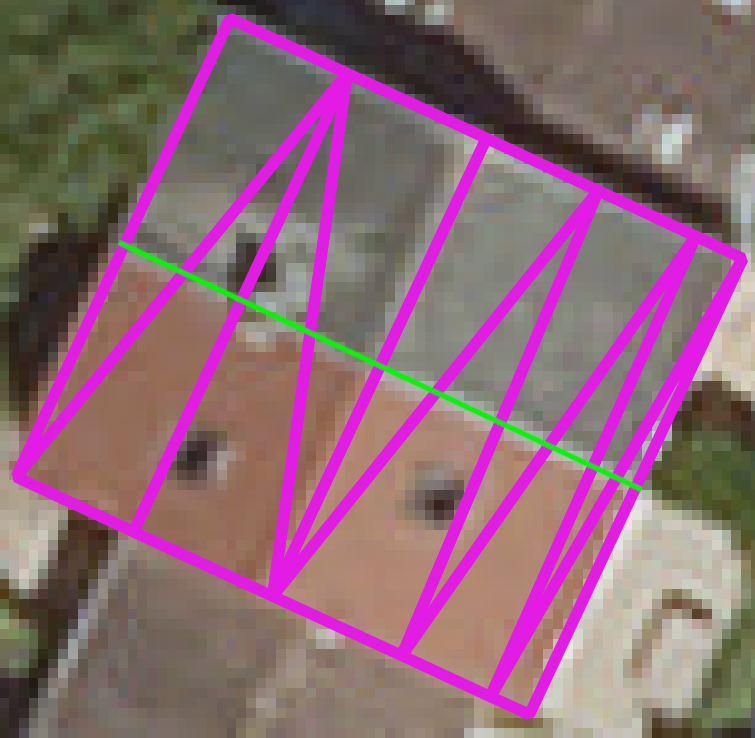
\includegraphics[height=.45\textheight]{images/errors/building/under_segmentation}}
                                \caption{\label{fig::bul_under} Under segmentation (\texttt{BUS}).}
                            \end{subfigure}
                            \begin{subfigure}{.5\textwidth}
                                \centering
                                \fbox{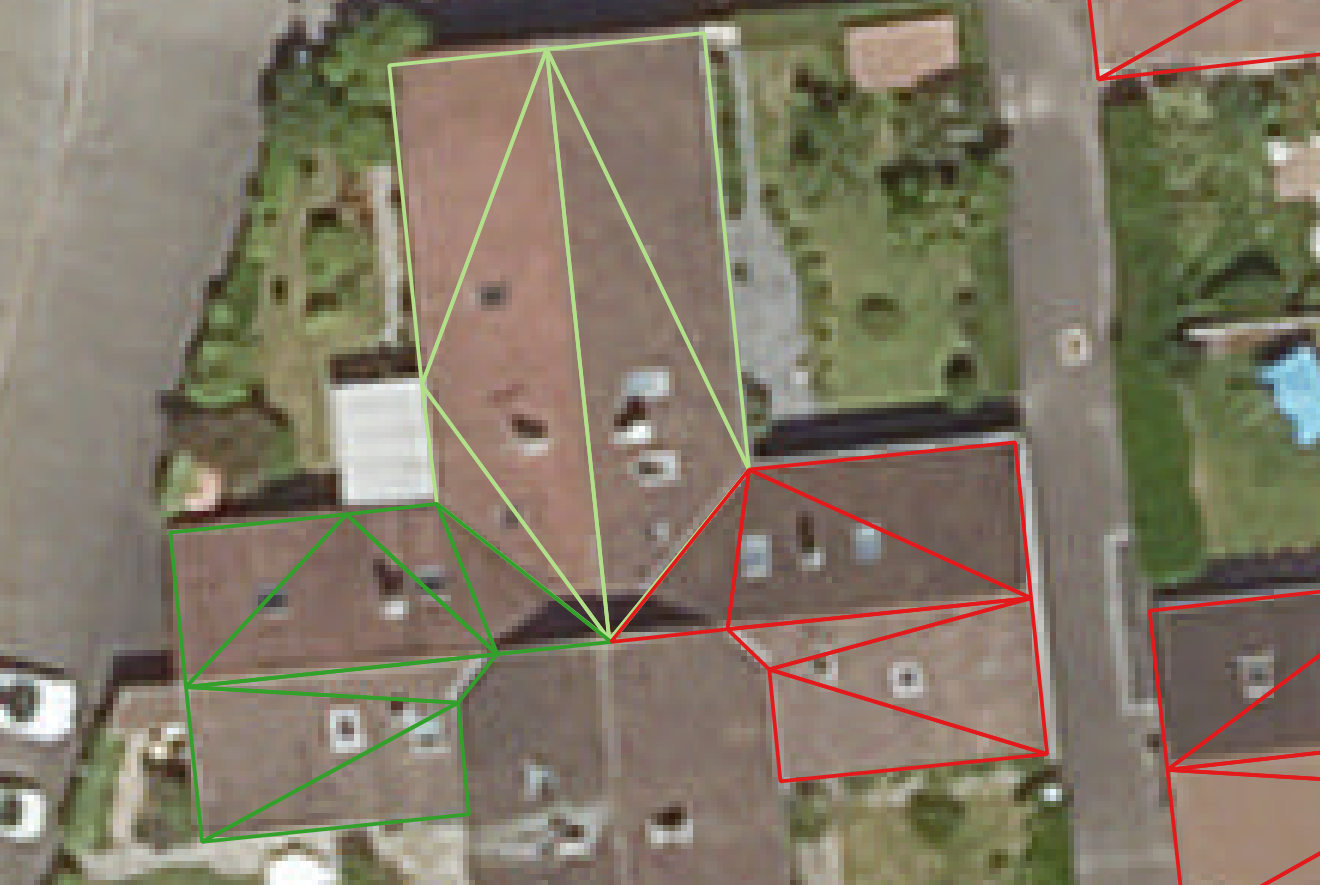
\includegraphics[height=.45\textheight]{images/errors/building/over_segmentation}}
                                \caption{\label{fig::bul_over} Over segmentation (\texttt{BOS}).}
                            \end{subfigure}
                        \end{center}
                    \end{figure}
                }
                \only<2|handout:2>{
                    \begin{figure}
                        \begin{center}
                            \begin{subfigure}{.45\textwidth}
                                \centering
                                \fbox{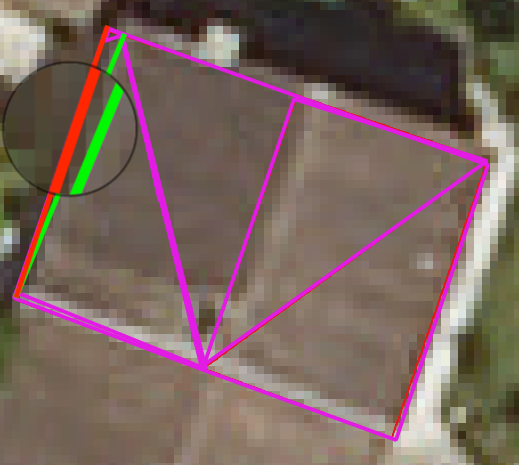
\includegraphics[height=.5\textheight]{images/errors/building/border}}
                                \caption{\label{fig::bul_footprint} Imprecise border (\texttt{BIB}).}
                            \end{subfigure}
                            \begin{subfigure}{.45\textwidth}
                                \centering
                                \fbox{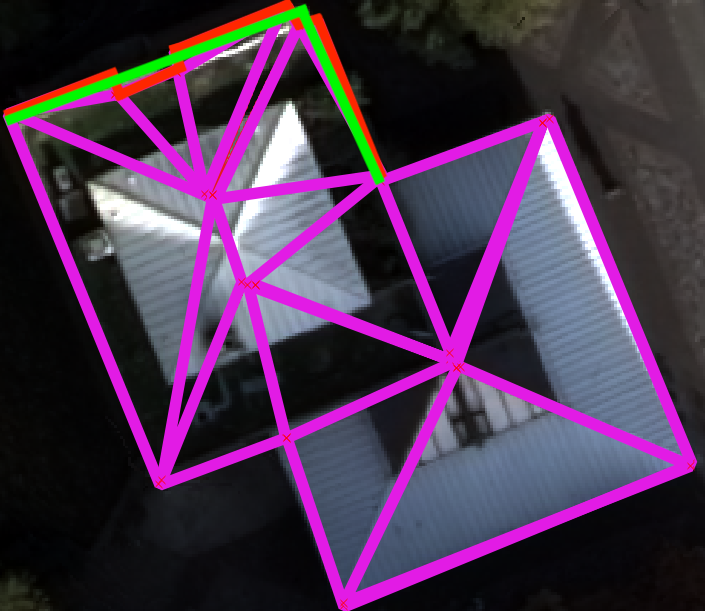
\includegraphics[height=.5\textheight]{images/errors/building/topology}}
                                \caption{\label{fig::bul_height} Inaccurate topology (\texttt{BIT}).}
                            \end{subfigure}
                        \end{center}
                    \end{figure}
                }
            \end{frame}
            \begin{frame}{Error taxonomy (\texttt{finesse} $= 3$, $\leq$ \acrshort{acr::lod}-2)}
                \begin{figure}
                    \includestandalone[mode=buildmissing, width=\textwidth]{finesse_3_all_taxonomy}
                \end{figure}
            \end{frame}
            \begin{frame}{Facet \texttt{atomic} errors: 2.5D overhead reconstruction case}
                \only<1|handout:1>{
                    \begin{figure}
                        \begin{center}
                            \begin{subfigure}{.31\textwidth}
                                \centering
                                \fbox{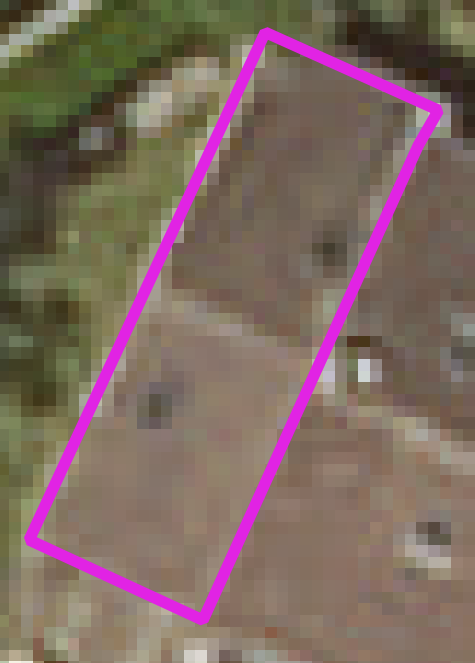
\includegraphics[height=.4\textheight]{images/errors/facet/under_segmentation}}
                                \caption{\label{fig::fac_under} Under segmentation (\texttt{FUS})}
                            \end{subfigure}
                            \begin{subfigure}{.31\textwidth}
                                \centering
                                \fbox{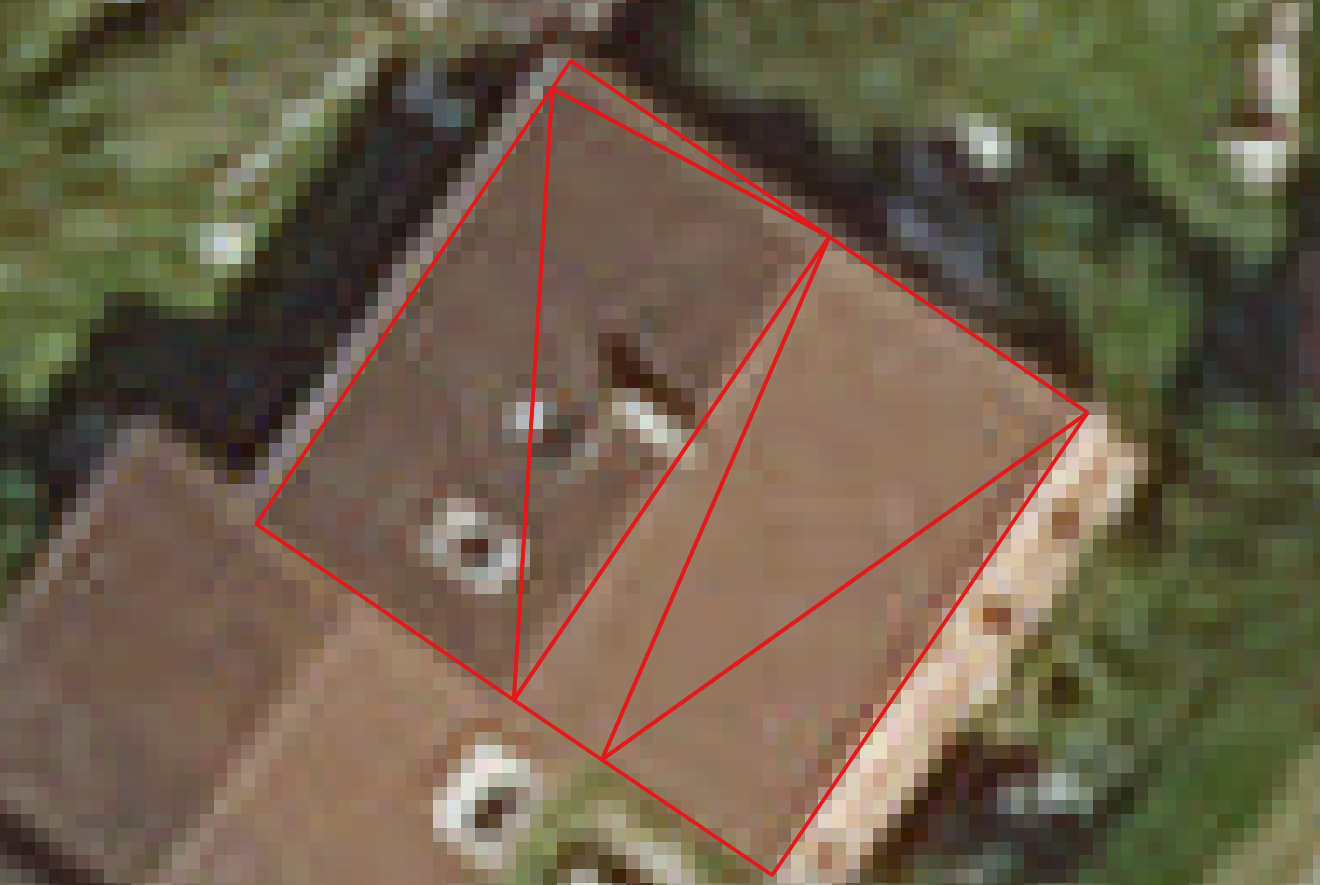
\includegraphics[height=.4\textheight]{images/errors/facet/over_segmentation}}
                                \caption{\label{fig::fac_over} Over segmentation (\texttt{FOS})}
                            \end{subfigure}
                            \begin{subfigure}{.31\textwidth}
                                \centering
                                \fbox{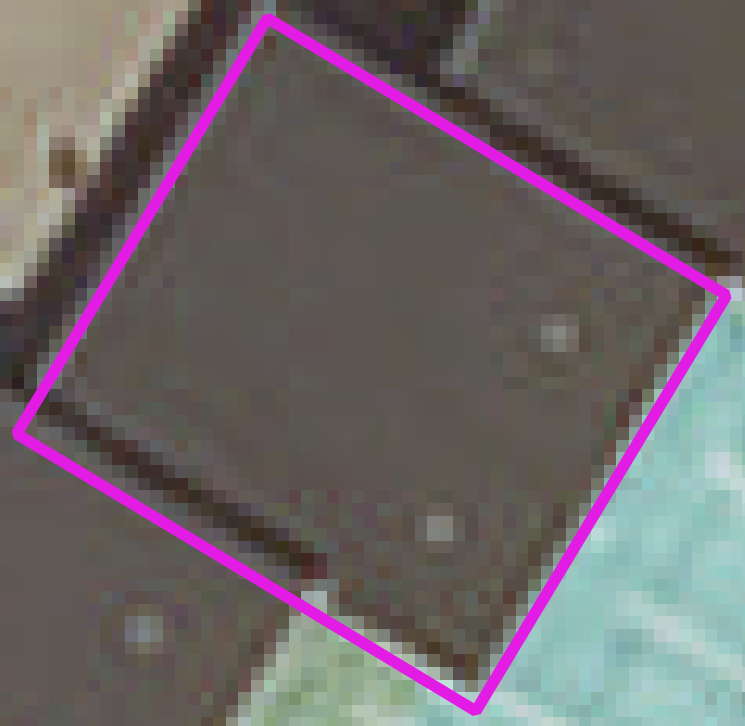
\includegraphics[height=.4\textheight]{images/errors/facet/geometry}}
                                \caption{\label{fig::fac_height} Imprecise geometry (\texttt{FIG})}
                            \end{subfigure}
                        \end{center}
                    \end{figure}
                }
                \only<2|handout:2>{
                    \begin{figure}
                        \begin{center}
                            \begin{subfigure}{.45\textwidth}
                                \centering
                                \fbox{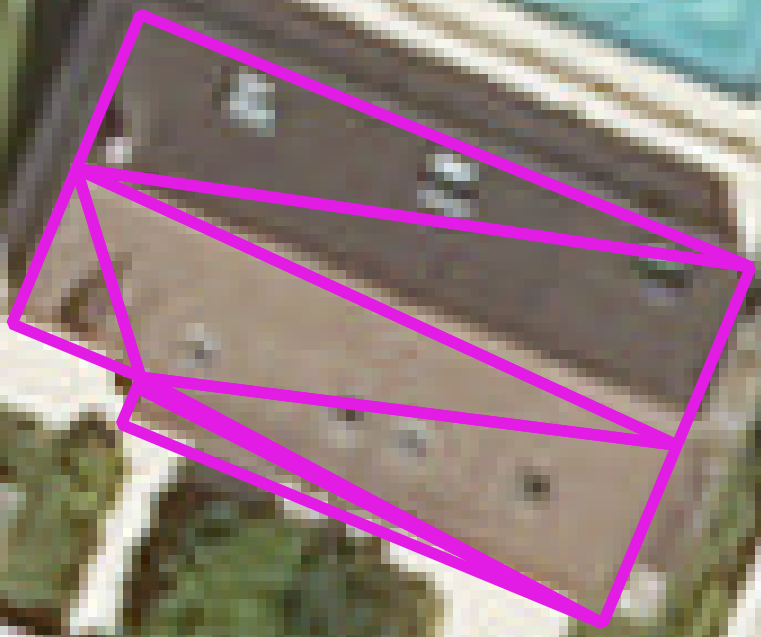
\includegraphics[height=.65\textwidth]{images/errors/facet/border}}
                                \caption{\label{fig::fac_footprint} Imprecise borders (\texttt{FIB})}
                            \end{subfigure}
                            \begin{subfigure}{.45\textwidth}
                                \centering
                                \fbox{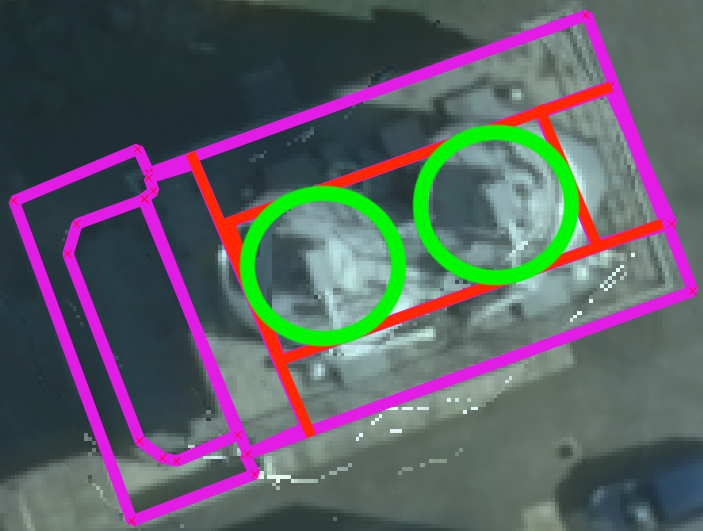
\includegraphics[height=.65\textwidth]{images/errors/facet/topology}}
                                \caption{\label{fig::fac_height} Inaccurate topology (\texttt{FIT})}
                            \end{subfigure}
                        \end{center}
                    \end{figure}
                }
            \end{frame}
        \subsection{Quality prediction pipeline}
            \begin{frame}{The evaluation pipeline}
                \begin{figure}
                    \includestandalone[mode=buildnew, height=.75\textheight]{graphical_abstract}
                \end{figure}
            \end{frame}
            \begin{frame}{Geometric features}
                \begin{figure}
                    \includestandalone[mode=buildnew, height=.62\textheight]{geometric_features}
                \end{figure}
                \begin{itemize}[label=$\blacktriangleright$, font=\color{IGNGreen}]
                    \item<2-> \footnotesize Statistics are computed, for each \underline{attribute}, at \underline{building} level.
                    \item<3-> \footnotesize Results are concatenated in a \underline{fixed size} feature vector (\textit{length = 20} in experiments).
                \end{itemize}
            \end{frame}
            \begin{frame}{Height-based features}
                \begin{figure}
                    \includestandalone[mode=buildnew, width=\textwidth]{altimetric_features}
                \end{figure}
                \begin{itemize}[label=$\blacktriangleright$, font=\color{IGNGreen}]
                    \item<2-> \footnotesize Feature vectors consist on the concatenated histogram values.
                    \item<3-> \footnotesize The histogram resolution is \underline{constant} (\textit{length = 20} in experiments).
                \end{itemize}
            \end{frame}
            \begin{frame}{Image-based features}
                \begin{figure}
                    \begin{center}
                        \includestandalone[mode=buildnew, width=.9\textwidth]{radiometric_features}
                    \end{center}
                \end{figure}
                \begin{itemize}[label=$\blacktriangleright$, font=\color{IGNGreen}]
                    \item<2-> \footnotesize A \underline{histogram} of the cosine similarity is computed \underline{per edge}.
                    \item<3-> \footnotesize A \underline{weighted sum} of all edge histograms is computed \underline{over the building}.
                    \item<4-> \footnotesize All histograms having the same resolution result in a feature vector (\textit{length = 20} in experiments).
                \end{itemize}
            \end{frame}
    \section{Experiments}
        \begin{frame}{Datasets: urban scenes}
            \begin{figure}
                \begin{center}
                    \includestandalone[mode=buildnew, width=.9\textwidth]{dataset}
                \end{center}
            \end{figure}
        \end{frame}
        \begin{frame}{Datasets: errors occurences}
            \only<1|handout:1>{
                \begin{figure}
                    \begin{center}
                        \includestandalone[mode=buildmissing, width=.7\textwidth]{dataset_stats_building}
                    \end{center}
                \end{figure}
            }
            \only<2-|handout:2>{
                \begin{figure}
                    \begin{center}
                        \includestandalone[mode=buildmissing, width=.8\textwidth]{dataset_stats_facet}
                    \end{center}
                \end{figure}
            }
            \begin{itemize}[label=$\blacktriangleright$, font=\color{IGNGreen}]
                \item<3-> \footnotesize Errors are \underline{heterogeneously} represented in the datasets.
                \item<4-> \footnotesize The less frequent errors would raise serious learning problems.
            \end{itemize}
        \end{frame}
        \begin{frame}{Ablation study: Elancourt example}
            \begin{table}
                \scriptsize
                \begin{center}
                    \scriptsize
                    \begin{tabular}{|x{.5cm} | x{.8cm} x{.8cm} | x{.9cm} x{.9cm} | x{.8cm} x{.8cm} | x{.8cm} x{.8cm}|}
                        \hline
                        &\multicolumn{2}{x{1.6cm}|}{\textbf{Geom.}} & \multicolumn{2}{x{1.8cm}|}{\textbf{Geom. $\cup$ Hei.}} & \multicolumn{2}{x{1.6cm}|}{\textbf{Geom. $\cup$ Im.}} & \multicolumn{2}{x{1.6cm}|}{\textbf{All}}\\
                        \cline{2-9}
                        &\textbf{Rec.} & \textbf{Prec.} & \textbf{Rec.} & \textbf{Prec.} & \textbf{Rec.} & \textbf{Prec.} & \textbf{Rec.} & \textbf{Prec.}\\
                        \hline
                        \texttt{BOS} & \textbf{93.96} & 76.15 & 91.43 & \textbf{77.76} & 91.51 & 76.08 & 90.83 & 76.14 \\
                        \hline
                        \strut\\[-\normalbaselineskip]
                        \only<3|handout:0>{\\[-\normalbaselineskip]\rowcolor{IGNGreen}}\texttt{BUS} & 32.98 & \textbf{76.47} & \textbf{41.86} & 75.57 & 40.38 & 71.00 & 39.32 & 71.81 \\
                        \hline
                        \strut\\[-\normalbaselineskip]
                        \only<5|handout:0>{\\[-\normalbaselineskip]\rowcolor{yellow}}\texttt{BIB} & 12.32 & 67.57 & 12.81 & \textbf{68.42} & 16.26 & 67.35 & \textbf{16.75} & 68.0 \\
                        \hline
                        \strut\\[-\normalbaselineskip]
                        \only<4|handout:0>{\\[-\normalbaselineskip]\rowcolor{IGNRed}}\only<5|handout:0>{\\[-\normalbaselineskip]\rowcolor{yellow}}\texttt{BIT} & \textbf{25.25} & 92.59 & 20.20 & 90.91 & 20.20 & \textbf{95.24} & 11.11 & 91.67 \\
                        \hline
                        \hline
                        \texttt{FOS} & 98.91 & 99.07 & 98.91 & \textbf{99.30} & \textbf{98.99} & 98.84 & 98.91 & 98.84 \\
                        \hline
                        \strut\\[-\normalbaselineskip]
                        \only<5|handout:0>{\\[-\normalbaselineskip]\rowcolor{yellow}}\texttt{FUS} & \textbf{1.90} & 54.55 & 0.63 & \textbf{66.67} & 1.61 & 50 & 1.27 & \textbf{66.67} \\
                        \hline
                        \strut\\[-\normalbaselineskip]
                        \only<5|handout:0>{\\[-\normalbaselineskip]\rowcolor{yellow}}\texttt{FIB} & \textbf{9.17} & 87.5 & 0 & --- & 8.30 & 82.61 & 7.42 & \textbf{100} \\
                        \hline
                        \strut\\[-\normalbaselineskip]
                        \only<5|handout:0>{\\[-\normalbaselineskip]\rowcolor{yellow}}\texttt{FIT} & \textbf{6.67} & \textbf{100} & 8.73 & 95.24 & 3.33 & \textbf{100} & 3.33 & \textbf{100} \\
                        \hline
                        \texttt{FIG} & \textbf{80.54} & 73.14 & 80.45 & \textbf{72.62} & 78.69 & 72.12 & 79.02 & 71.82 \\
                        \hline
                    \end{tabular}
                \end{center}
            \end{table}
            \only<1>{
                \begin{center}
                    \footnotesize Results in percentage obtained using \texttt{RF} (\underline{1,000 trees} \& \underline{max depth 4}) and \underline{10-fold cross. val}.
                \end{center}
            }
            \begin{itemize}[label=$\blacktriangleright$, font=\color{IGNGreen}]
                \item<2-> \footnotesize In most cases \textbf{Geom.} is sufficient;
                \item<3-> \footnotesize Except for \texttt{BUS} $\rightarrow$ other modalities have a big impact ($\approx$ + 10\%).
                \item<4-> \footnotesize Only \textbf{Geom.} is even \underline{the best} for \texttt{BIT}.
                \item<5-> \footnotesize Highly unbalanced labels are \underline{hard} to detect.
            \end{itemize}
        \end{frame}
        \begin{frame}{Feature importance}
            \only<1|handout:0>{
                \begin{itemize}[label=$\blacktriangleright$, font=\color{IGNGreen}]
                    \item<1> Does this mean additional modalities are useless?
                \end{itemize}
            }
            \only<2|handout:1>{
                \begin{figure}
                    \includestandalone[mode=buildnew, width=.846\textwidth]{feat_imp_building}
                \end{figure}
            }
            \only<3|handout:2>{
                \begin{figure}
                    \includestandalone[mode=buildnew, width=\textwidth]{feat_imp_facet}
                \end{figure}
            }
            \only<4-|handout:3>{
                \begin{itemize}[label=$\blacktriangleright$, font=\color{IGNGreen}, itemsep=2em]
                    \item<4-> All features importances contribute \underline{equally} around 33\%.
                    \item<5-> When do these additional features play a role?
                \end{itemize}
            }
        \end{frame}
        \begin{frame}{Scalability study: conducted experimentations}
            \begin{figure}
                \includestandalone[mode=buildnew, height=.7\textheight]{scalabitity_graph}
            \end{figure}
            \only<2|handout:0>{
                \begin{itemize}[label=$\blacktriangleright$, font=\color{IGNGreen}]
                    \item \footnotesize Transferability: train on \underline{one} scene and test on a different \underline{one}.
                \end{itemize}
            }
            \only<3|handout:0>{
                \begin{itemize}[label=$\blacktriangleright$, font=\color{IGNGreen}]
                    \item \footnotesize Generalization: train on \underline{two} scenes and test on the \underline{one} leftout.
                \end{itemize}
            }
            \only<4|handout:0>{
                \begin{itemize}[label=$\blacktriangleright$, font=\color{IGNGreen}]
                    \item \footnotesize Representativeness: train on \underline{different fractions} of the \underline{combined} scenes.
                \end{itemize}
            }
        \end{frame}
        \begin{frame}{Transferability}
            \only<1|handout:1>{
                \begin{table}
                    \scriptsize
                    \begin{center}
                        \begin{tabular}{| x{1.5cm}| x{.4cm} | x{.4cm} | x{.4cm} | x{.4cm} | x{.4cm} | x{.4cm} | x{.4cm} | x{.4cm} | x{.4cm} |}
                            \hline
                            &\texttt{BOS}  & \texttt{BUS} &\texttt{BIB} &\texttt{BIT} &\texttt{FOS}  & \texttt{FUS} &\texttt{FIB} &\texttt{FIT} &\texttt{FIG} \\
                            \hline
                            Elancourt $\rightarrow$ Nantes &\cellcolor{Moins1} & \cellcolor{Moins2}&\cellcolor{Moins1}& \cellcolor{Moins2}& \cellcolor{Zero}& \cellcolor{Zero}&\cellcolor{Plus2} Im. & \cellcolor{Moins1}&\cellcolor{Zero}\\
                            \hline
                            Elancourt $\rightarrow$ Paris-13  & \cellcolor{Moins1}& \cellcolor{Moins2}& \cellcolor{Zero}& \cellcolor{Moins2}& \cellcolor{Zero}& \cellcolor{Plus1}Im.& \cellcolor{Plus1}Im.& \cellcolor{Moins1}&\cellcolor{Zero}\\
                            \hline
                            Nantes $\rightarrow$ Paris-13  & \cellcolor{Moins1}& \cellcolor{Moins2}& \cellcolor{black} & \cellcolor{Plus2}& \cellcolor{Zero}& \cellcolor{Plus1}& \cellcolor{Plus1}& \cellcolor{black} &\cellcolor{Zero}\\
                            \hline
                            Nantes $\rightarrow$ Elancourt  &\cellcolor{Plus1} & \cellcolor{Moins1}& \cellcolor{Moins1}&\cellcolor{Plus1}All & \cellcolor{Zero}& \cellcolor{Moins2}&\cellcolor{Moins1}Im. &\cellcolor{Plus1}Im. &\cellcolor{Zero}\\
                            \hline
                            Paris-13 $\rightarrow$ Nantes  &\cellcolor{Moins2} & \cellcolor{Moins1}& \cellcolor{black} & \cellcolor{Plus1}&\cellcolor{Zero} & \cellcolor{Moins3}& \cellcolor{Zero}& \cellcolor{black} & \cellcolor{Moins1} Hei.\\
                            \hline
                            Paris-13 $\rightarrow$ Elancourt &\cellcolor{Zero} &\cellcolor{Moins1} & \cellcolor{Plus1}Im. & \cellcolor{Zero}& \cellcolor{Zero}& \cellcolor{Moins4}& \cellcolor{Moins2}Im. & \cellcolor{black} & \cellcolor{Zero}\\
                            \hline
                        \end{tabular}
                    \end{center}
                \end{table}
                \begin{center}
                    \begin{tikzpicture}
                        \shade[left color=white,right color=Moins4] (0, 0) rectangle (1, .25);
                        \draw[Moins4, fill=Moins4] (1, 0) rectangle (2, .25);
                        \draw[Moins3, fill=Moins3] (2, 0) rectangle (3, .25);
                        \draw[Moins2, fill=Moins2] (3, 0) rectangle (4, .25);
                        \draw[Moins1, fill=Moins1] (4, 0) rectangle (5, .25);
                        \draw[Zero, fill=Zero] (5, 0) rectangle (6, .25);
                        \draw[Plus1, fill=Plus1] (6, 0) rectangle (7, .25);
                        \draw[Plus2, fill=Plus2] (7, 0) rectangle (8, .25);
                        \shade[left color=Plus2,right color=white] (8, 0) rectangle (9, .25);
                        \draw[black] (0, 0) -- (9, 0);
                        \draw[black] (0, .25) -- (9, .25);
                        \draw[black, fill=black] (5, -.75) rectangle (4, -1);
                        \path (4.5, -1.25) node {\footnotesize NaN};
                        \draw[black] (1, .25) -- (1, -2pt) node[below, IGNDarkGrey] {\footnotesize -45\%};
                        \draw[black] (2, .25) -- (2, -2pt) node[below, IGNDarkGrey] {\footnotesize -35\%};
                        \draw[black] (3, .25) -- (3, -2pt) node[below, IGNDarkGrey] {\footnotesize -25\%};
                        \draw[black] (4, .25) -- (4, -2pt) node[below, IGNDarkGrey] {\footnotesize -15\%};
                        \draw[black] (5, .25) -- (5, -2pt) node[below, IGNDarkGrey] {\footnotesize -5\%};
                        \draw[black] (6, .25) -- (6, -2pt) node[below, IGNDarkGrey] {\footnotesize 5\%};
                        \draw[black] (7, .25) -- (7, -2pt) node[below, IGNDarkGrey] {\footnotesize 15\%};
                        \draw[black] (8, .25) -- (8, -2pt) node[below, IGNDarkGrey] {\footnotesize 25\%};
                    \end{tikzpicture}
                \end{center}
            }
            \only<2-|handout:2>{
                \begin{table}
                    \scriptsize
                    \begin{center}
                        \begin{tabular}{| x{1.5cm}| x{.4cm} | x{.4cm} | x{.4cm} | x{.4cm} | x{.4cm} | x{.4cm} | x{.4cm} | x{.4cm} | x{.4cm} |}
                            \hline
                            &\texttt{BOS}  & \texttt{BUS} &\texttt{BIB} &\texttt{BIT} &\texttt{FOS}  & \texttt{FUS} &\texttt{FIB} &\texttt{FIT} &\texttt{FIG} \\
                            \hline
                            Elancourt $\rightarrow$ Nantes &\cellcolor{IGNRed} & \cellcolor{IGNRed}&\cellcolor{IGNRed}& \cellcolor{IGNRed}& \cellcolor{IGNGreen}& \cellcolor{IGNGreen}&\cellcolor{IGNGreen} Im. & \cellcolor{IGNRed}&\cellcolor{IGNGreen}\\
                            \hline
                            Elancourt $\rightarrow$ Paris-13  & \cellcolor{IGNRed}& \cellcolor{IGNRed}& \cellcolor{IGNGreen}& \cellcolor{IGNRed}& \cellcolor{IGNGreen}& \cellcolor{IGNGreen}Im.& \cellcolor{IGNGreen}Im.& \cellcolor{IGNRed}&\cellcolor{IGNGreen}\\
                            \hline
                            Nantes $\rightarrow$ Paris-13  & \cellcolor{IGNRed}& \cellcolor{IGNRed}& \cellcolor{black} & \cellcolor{IGNGreen}& \cellcolor{IGNGreen}& \cellcolor{IGNGreen}& \cellcolor{IGNGreen}& \cellcolor{black} &\cellcolor{IGNGreen}\\
                            \hline
                            Nantes $\rightarrow$ Elancourt  &\cellcolor{IGNGreen} & \cellcolor{IGNRed}& \cellcolor{IGNRed}&\cellcolor{IGNGreen}All & \cellcolor{IGNGreen}& \cellcolor{IGNRed}&\cellcolor{IGNRed}Im. &\cellcolor{IGNGreen}Im. &\cellcolor{IGNGreen}\\
                            \hline
                            Paris-13 $\rightarrow$ Nantes  &\cellcolor{IGNRed} & \cellcolor{IGNRed}& \cellcolor{black} & \cellcolor{IGNGreen}&\cellcolor{IGNGreen} & \cellcolor{IGNRed}& \cellcolor{IGNGreen}& \cellcolor{black} & \cellcolor{IGNRed} Hei.\\
                            \hline
                            Paris-13 $\rightarrow$ Elancourt &\cellcolor{IGNGreen} &\cellcolor{IGNRed} & \cellcolor{IGNGreen}Im. & \cellcolor{IGNGreen}& \cellcolor{IGNGreen}& \cellcolor{IGNRed}& \cellcolor{IGNRed}Im. & \cellcolor{black} & \cellcolor{IGNGreen}\\
                            \hline
                        \end{tabular}
                        \caption{\footnotesize \textcolor{IGNRed}{$\blacksquare$}: Loss in F-score, \textcolor{IGNGreen}{$\blacksquare$}: Stability or gain in F-score.}
                    \end{center}
                \end{table}
                \begin{itemize}[label=$\blacktriangleright$, font=\color{IGNGreen}]
                    \item<2-> \footnotesize Only 8/24 of \texttt{Building errors} transferability cases are \textcolor{IGNGreen}{positive}.
                    \item<3-> \footnotesize \texttt{Facets errors} are more transferable: 19/30 are \textcolor{IGNGreen}{positive}.
                \end{itemize}
            }
        \end{frame}
        \begin{frame}{Generalization}
            \only<1|handout:1>{
                \begin{table}
                    \scriptsize
                    \begin{center}
                        \begin{tabular}{| x{1.5cm}| x{.4cm} | x{.4cm} | x{.4cm} | x{.4cm} | x{.4cm} | x{.4cm} | x{.4cm} | x{.4cm} | x{.4cm} |}
                            \hline
                            &\texttt{BOS}  & \texttt{BUS} &\texttt{BIB} &\texttt{BIT} &\texttt{FOS}  & \texttt{FUS} &\texttt{FIB} &\texttt{FIT} &\texttt{FIG} \\
                            \hline
                            Nnt. $\cup$ P-13 $\rightarrow$ Elancourt & \cellcolor{Moins2}& \cellcolor{Moins2}Im.& \cellcolor{Moins2}&\cellcolor{Moins2} &\cellcolor{Zero} &\cellcolor{Plus1}Im. &\cellcolor{Plus2}Im. &\cellcolor{Moins1}Geo & \cellcolor{Moins1} Hei\\
                            \hline
                            El. $\cup$ P-13 $\rightarrow$ Nantes & \cellcolor{Zero}All& \cellcolor{Moins2}Im.&\cellcolor{Moins1}Im. &\cellcolor{Plus2} &\cellcolor{Zero} & \cellcolor{Zero}& \cellcolor{Moins2}Im.& \cellcolor{black} &\cellcolor{Zero}\\
                            \hline
                            El. $\cup$ Nnt. $\rightarrow$ Paris-13 &\cellcolor{Moins2}All &\cellcolor{Moins2} & \cellcolor{black} &\cellcolor{Plus1}Hei. &\cellcolor{Zero} &\cellcolor{Moins4} &\cellcolor{Moins2}Im. & \cellcolor{black} &\cellcolor{Moins1}\\
                            \hline
                        \end{tabular}
                    \end{center}
                \end{table}
                \begin{center}
                    \begin{tikzpicture}
                        \shade[left color=white,right color=Moins4] (0, 0) rectangle (1, .25);
                        \draw[Moins4, fill=Moins4] (1, 0) rectangle (2, .25);
                        \draw[Moins3, fill=Moins3] (2, 0) rectangle (3, .25);
                        \draw[Moins2, fill=Moins2] (3, 0) rectangle (4, .25);
                        \draw[Moins1, fill=Moins1] (4, 0) rectangle (5, .25);
                        \draw[Zero, fill=Zero] (5, 0) rectangle (6, .25);
                        \draw[Plus1, fill=Plus1] (6, 0) rectangle (7, .25);
                        \draw[Plus2, fill=Plus2] (7, 0) rectangle (8, .25);
                        \shade[left color=Plus2,right color=white] (8, 0) rectangle (9, .25);
                        \draw[black] (0, 0) -- (9, 0);
                        \draw[black] (0, .25) -- (9, .25);
                        \draw[black, fill=black] (5, -.75) rectangle (4, -1);
                        \path (4.5, -1.25) node {\footnotesize NaN};
                        \draw[black] (1, .25) -- (1, -2pt) node[below, IGNDarkGrey] {\footnotesize -45\%};
                        \draw[black] (2, .25) -- (2, -2pt) node[below, IGNDarkGrey] {\footnotesize -35\%};
                        \draw[black] (3, .25) -- (3, -2pt) node[below, IGNDarkGrey] {\footnotesize -25\%};
                        \draw[black] (4, .25) -- (4, -2pt) node[below, IGNDarkGrey] {\footnotesize -15\%};
                        \draw[black] (5, .25) -- (5, -2pt) node[below, IGNDarkGrey] {\footnotesize -5\%};
                        \draw[black] (6, .25) -- (6, -2pt) node[below, IGNDarkGrey] {\footnotesize 5\%};
                        \draw[black] (7, .25) -- (7, -2pt) node[below, IGNDarkGrey] {\footnotesize 15\%};
                        \draw[black] (8, .25) -- (8, -2pt) node[below, IGNDarkGrey] {\footnotesize 25\%};
                    \end{tikzpicture}
                \end{center}
            }
            \only<2-|handout:2>{
                \begin{table}
                    \scriptsize
                    \begin{center}
                        \begin{tabular}{| x{1.5cm}| x{.4cm} | x{.4cm} | x{.4cm} | x{.4cm} | x{.4cm} | x{.4cm} | x{.4cm} | x{.4cm} | x{.4cm} |}
                            \hline
                            &\texttt{BOS}  & \texttt{BUS} &\texttt{BIB} &\texttt{BIT} &\texttt{FOS}  & \texttt{FUS} &\texttt{FIB} &\texttt{FIT} &\texttt{FIG} \\
                            \hline
                            Nnt. $\cup$ P-13 $\rightarrow$ Elancourt & \cellcolor{IGNRed}& \cellcolor{IGNRed}Im.& \cellcolor{IGNRed}&\cellcolor{IGNRed} &\cellcolor{IGNGreen} &\cellcolor{IGNGreen}Im. &\cellcolor{IGNGreen}Im. &\cellcolor{IGNRed}Geo & \cellcolor{IGNRed} Hei\\
                            \hline
                            El. $\cup$ P-13 $\rightarrow$ Nantes   & \cellcolor{IGNGreen}All& \cellcolor{IGNRed}Im.&\cellcolor{IGNRed}Im. &\cellcolor{IGNGreen} &\cellcolor{IGNGreen} & \cellcolor{IGNGreen}& \cellcolor{IGNRed}Im.& \cellcolor{black} &\cellcolor{IGNGreen}\\
                            \hline
                            El. $\cup$ Nnt. $\rightarrow$ Paris-13   &\cellcolor{IGNRed}All &\cellcolor{IGNRed} & \cellcolor{black} &\cellcolor{IGNGreen}Hei. &\cellcolor{IGNGreen} &\cellcolor{IGNRed} &\cellcolor{IGNRed}Im. & \cellcolor{black} &\cellcolor{IGNRed}\\
                            \hline
                        \end{tabular}
                        \caption{\footnotesize \textcolor{IGNRed}{$\blacksquare$}: Loss in F-score, \textcolor{IGNGreen}{$\blacksquare$}: Stability or gain in F-score.}
                    \end{center}
                \end{table}
                \begin{itemize}[label=$\blacktriangleright$, font=\color{IGNGreen}]
                    \item<2-> \footnotesize Only 3/12 of \texttt{Building errors} generalization cases are \textcolor{IGNGreen}{positive}.
                    \item<3-> \footnotesize \texttt{Facets errors} are more generalizable: 7/15 are \textcolor{IGNGreen}{positive}.
                    \item<4-> \footnotesize More diverse training data \underline{averages out} results.
                \end{itemize}
            }
        \end{frame}
        \begin{frame}{Representativeness}
            \begin{figure}
                \includestandalone[mode=buildnew, height=.65\textheight]{f-scores_f3_repr}
            \end{figure}
            \begin{itemize}[label=$\blacktriangleright$, font=\color{IGNGreen}]
                \item<2-> \footnotesize F-scores are \textbf{stable} no matter how much the \underline{training set size} changes.
                \item<3-> \footnotesize Results are even \underline{more stable} for the \underline{very frequent} errors.
            \end{itemize}
        \end{frame}
        \begin{frame}{Some failure cases on Elancourt}
            \begin{figure}
                \begin{center}
                \tiny
                    \begin{tabular}{| x{.06\textwidth} | x{.035\textwidth} | x{.035\textwidth} || x{.06\textwidth} | x{.035\textwidth} | x{.035\textwidth} || x{.06\textwidth} | x{.035\textwidth} | x{.035\textwidth} || x{.06\textwidth} | x{.035\textwidth} | x{.035\textwidth} |}
                        \hline
                        \multicolumn{3}{| c ||}{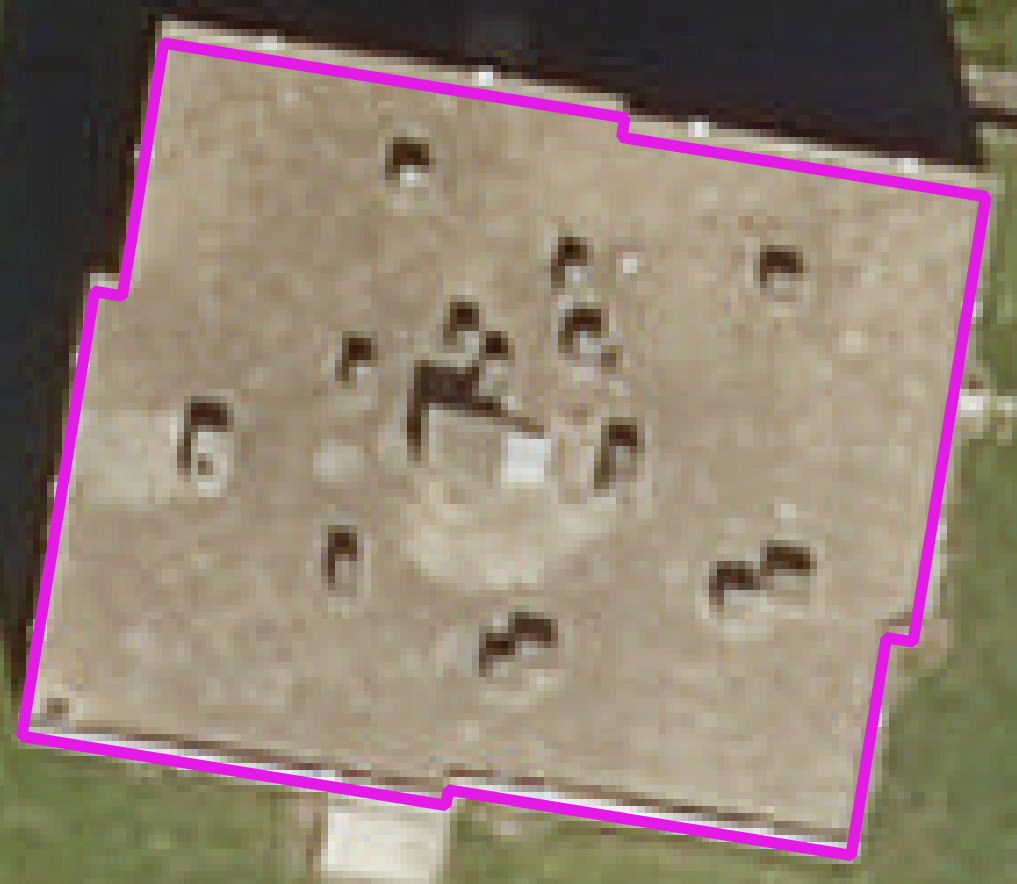
\includegraphics[width=.2\textwidth,valign=m,margin=1pt 1pt]{images/prediction_results/valid_as_bul_over}} & \multicolumn{3}{ c ||}{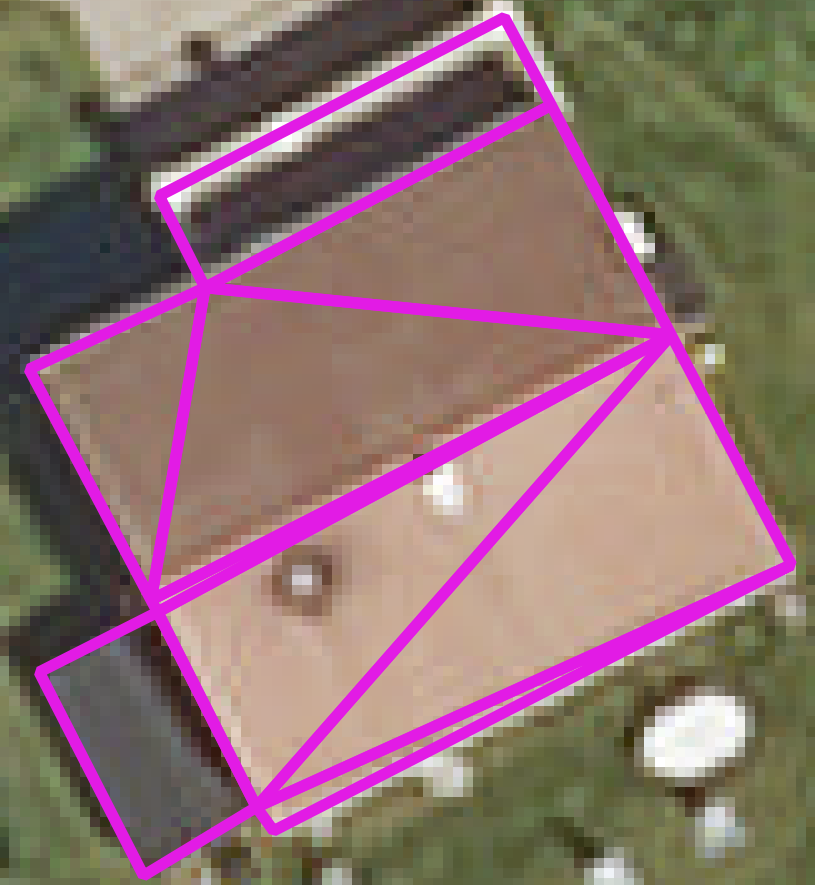
\includegraphics[width=.2\textwidth,valign=m,margin=0cm 1pt]{images/prediction_results/no_imprec_no_fac_over}} & \multicolumn{3}{ c ||}{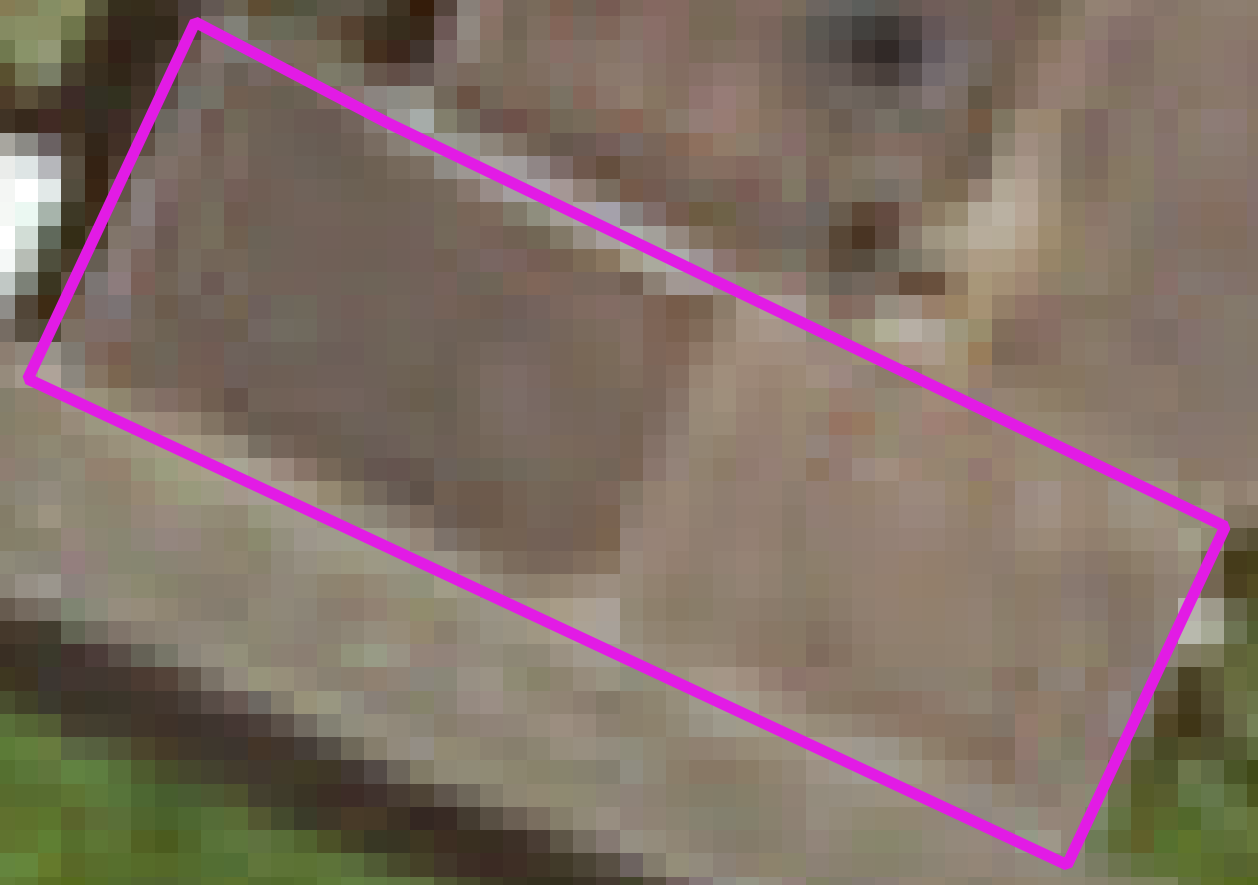
\includegraphics[width=.2\textwidth,valign=m,margin=0cm 1pt]{images/prediction_results/no_under_seg}} & \multicolumn{3}{ c |}{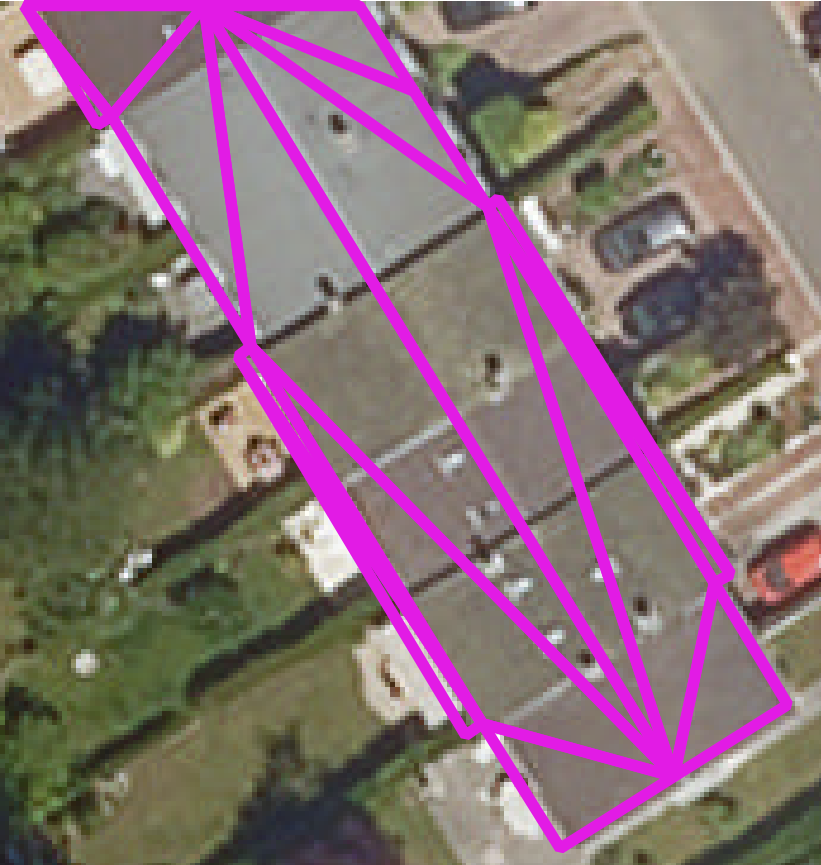
\includegraphics[width=.2\textwidth,valign=m,margin=0cm 1pt]{images/prediction_results/no_bul_under_seg}} \\
                        \hline
                        \textbf{Errors} & \textbf{G.T.} & \textbf{Pred.} & \textbf{Errors} & \textbf{G.T.} & \textbf{Pred.} & \textbf{Errors} & \textbf{G.T.} & \textbf{Pred.} & \textbf{Errors} & \textbf{G.T.} & \textbf{Pred.}\\
                        \hline
                        \texttt{BOS} & \xmark & \cmark & \texttt{BUS} & \xmark & \cmark & \texttt{BOS} & \cmark & \cmark & \texttt{BOS} & \cmark & \xmark \\
                         &  &  & \texttt{FIG} & \cmark & \xmark & \texttt{FUS} & \cmark & \xmark &  \texttt{FOS} & \cmark & \xmark \\
                            &  &  & \texttt{FOS} & \cmark & \xmark &  &  &  & \texttt{BUS} & \cmark & \xmark \\
                            &  &  &  &  &  &  &  &  &  \texttt{BIB} & \cmark & \cmark \\
                        \hline
                    \end{tabular}
                \end{center}
            \end{figure}
        \end{frame}
        
    \section{Conclusion}
        \begin{frame}{\textcolor{yellow}{Conclusion} \& \textcolor{purple}{Perspectives}}
            \begin{itemize}[label=$\blacktriangleright$, font=\color{yellow}, itemsep=2em]
                \item<1-> \textbf{Flexible, robust and hierarchical} taxonomy;
                \item<2-> \textbf{Fast, lightweight and modular} pipeline for model evaluation;
                \item<3-> Pipeline tested with \textbf{baseline} handcrafted features:
                    \begin{itemize}[label=$\blacktriangleright$, font=\color{IGNGreen}]
                        \item<4-> Results limited by the lack of training data;
                        \item<5-> Need for a thorough representation of urban landscapes.
                    \end{itemize}
            \end{itemize}
            \uncover<6->{
                ~\\
                Future work:
                \begin{itemize}[label=$\blacktriangleright$, font=\color{purple}, itemsep=2em]
                    \item<6-> Extend to richer features $\longrightarrow$ Graph kernels, Scattering.
                    \item<7-> Dataset augmentation $\longrightarrow$ \textbf{Simulate errors}.
                \end{itemize}
            }
        \end{frame}
\end{document}
